% Define the document type and special pacages
%--------------------------------------------------------%
\documentclass[12pt]{article}
\usepackage[utf8]{inputenc}

\title{Reseach Course on Detector technology - Semiconductor detector}
\author{group 1}
\date{\today}

\usepackage{listings}
\usepackage{color}
\usepackage[pdftex]{graphicx}
\usepackage{siunitx} % SI units
\usepackage{amsmath} % equations
\usepackage{tabularx}
\usepackage{tikz}
\usepackage{hyperref}
\usepackage{ifthen}
\usepackage[T1]{fontenc} % proper underscores etc.
\usepackage{subcaption} % replace subfloat with subfigure env.
\sisetup{per-mode=fraction}


\begin{document}
% === Front matter ====================================================

%\frontmatter
\maketitle

\clearpage
  
\tableofcontents
  
%\listoffigures
  
%\listoftables
  
%\lstlistoflistings
  
\cleardoublepage

%################################################################################################
%
% Introduction
%
%################################################################################################

\section{Introduction}

Semiconductor detectors, in particular silicon detectors, are often used in particle physics detectors for charged track detection, an example being the SCT detector in the ATLAS experiment at CERN. But what makes semiconductor detectors special? And why are they so widely used?

A semiconductor is a material where the energy gap between the conduction band and the valence band is of the order of magnitude of $1$ eV. When a charge is detected, an ionizing current is created where freed electrons and holes move to the conduction and valence band respectively. Depending on the number of freed electrons, one can deduct the energy of the charge detected. The detection of the energy is very fast in semiconductor detector, as electrons move fast, and it is spacially very precise, especially when an electric field is applied to the detector, making the charges go to the anode and cathode to be measured.

All of this makes semiconductor detectors very attractive for particle level detection.
In this experiment the production of a semiconductor detector is followed, the resulting diode is characterised and then connected to a pre-amplifier, in order to study the response of this silicon diode to a radioactive source.

%################################################################################################
%
% Experimental setup
%
%################################################################################################

\section{Experimental setup}

We worked on a p-type silicon detector. The device was exposed to a soft X-ray source and operated under a bias that ensured depletion of the entire chip. Depletion means that there are no intrinsic charge carrier left on the device, so all the signal measured will come from photoexcitation plus noise from the electronics. The silicon chip was provided without any connection between the top and bottom electrodes. To make these connections, the chip was sent to a clean room where wires were ultrasonically bonded to the top of the chip and the side electrode contacts.

Once the wire bonding was done, the sensor was placed inside a dark room workstation and its basic performances were evaluated. First, a calibration run measures the parasitic capacitance between the two contacts (in this case needles) of the sensor. Next, a voltage bias scan is performed, and the leakage current is measured with a pico amp-meter until we reach a plateau that corresponds to the depletion voltage. Finally the capacitance of the sensor is measured as a function of voltage and the parasitic capacitance is subtracted, to get the correct value of the capacitance of the silicon detector.

\begin{figure}[htb]
  \centering
  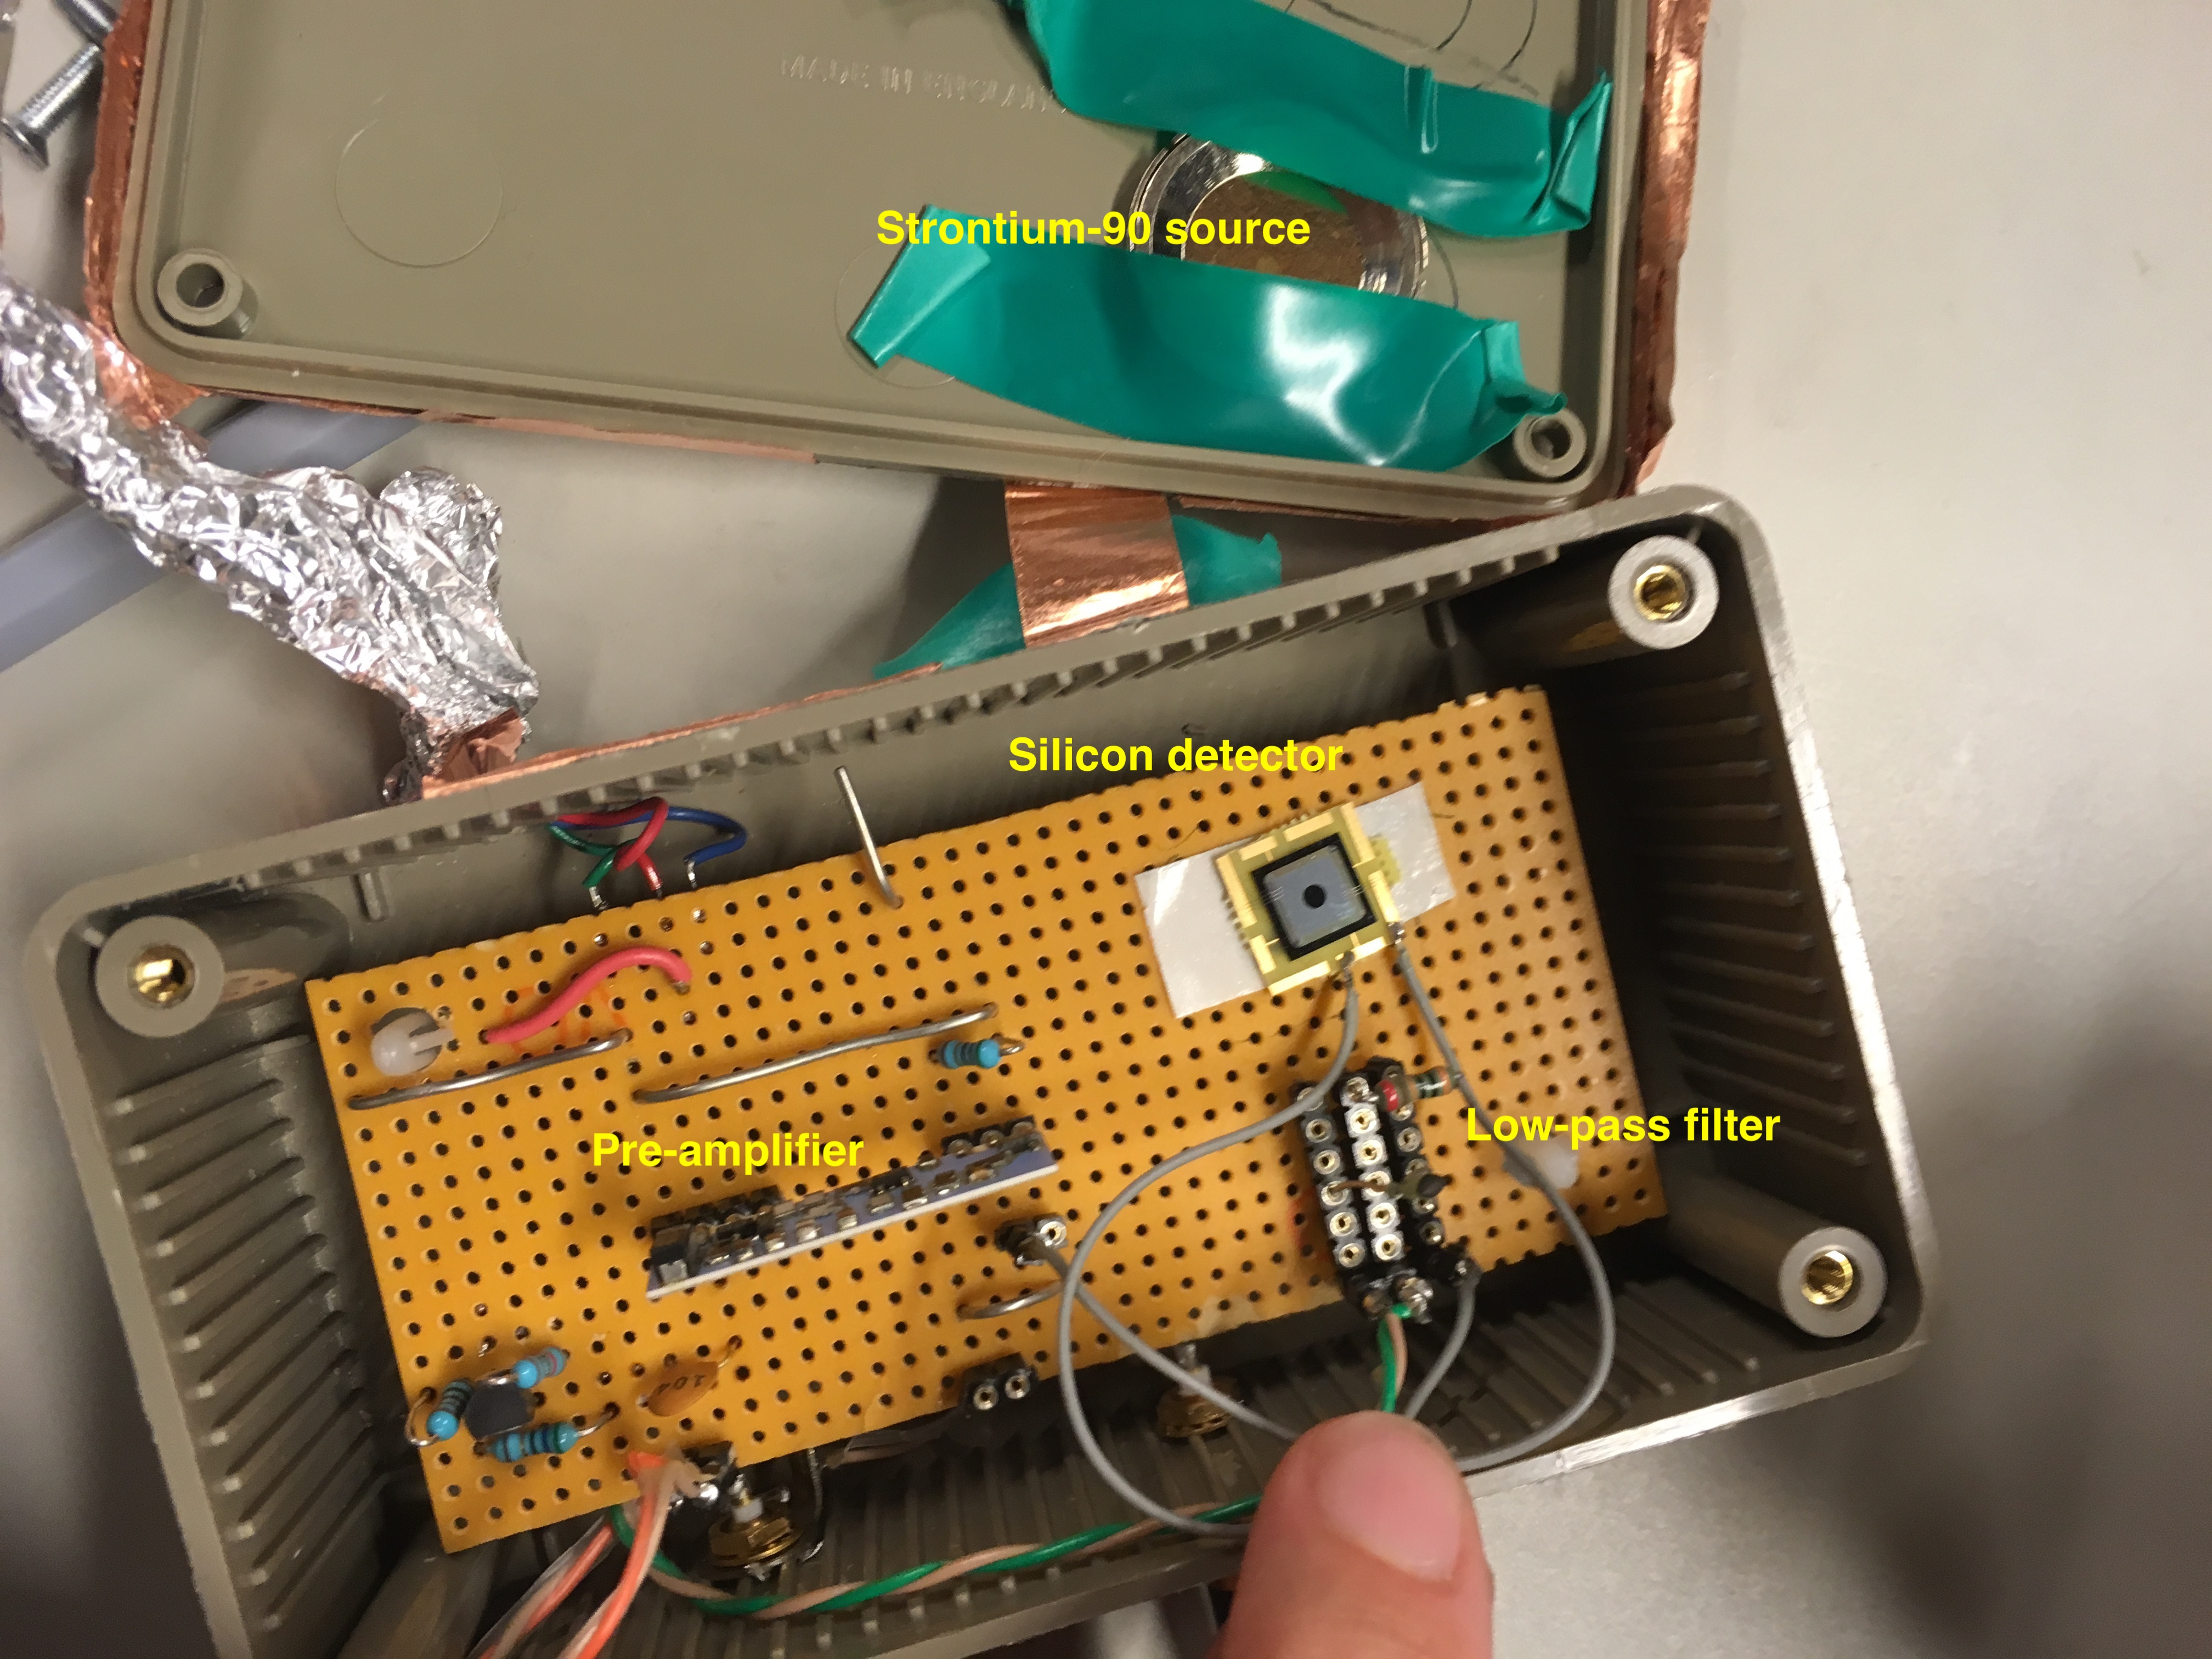
\includegraphics[width=0.8\textwidth]{./graphics/experimentalSetup}
  \caption{Silicon detector experimental setup.}
  \label{fig:ExperimentalSetup}
\end{figure}

Before attaching the sensor to the rest of the circuit to perform measurements, the response of the pre-amplifier was calibrated using different capacitances between $1$ pF and $100$ pF put in parallel to the capacitance of $0.4$ pF at the calibration input. To do this, the amplifier was supplied with two voltage biases of + and -12V from a DC workbench power supply. The RMS of the baseline noise was measured while no pulse was injected. The circuit was fed with a square pulse and the rise time of the output signal was measured directly on the oscilloscope between the $10\%$ and $90\%$ of the rising signal. The amplitude of the signal was noted as well. During these measurements, the circuit and the cables were coated with aluminium foil (grounded through a cable to the HV power supply), in order to shield the system from radiations, which would cause additional noise to the output signal.

After the calibration measurements were completed, the silicon detector was introduced in the circuit by connecting it to the pre-amplifier. A voltage of around $60$ V was fed to the sensor, in order to fully deplete it, through a low-pass filter consisting of a $100$ nF capacitance and of a $300$ k$\Omega$ resistor, see Figure \ref{fig:ExperimentalSetup}. The resulting circuit is schematically shown in Figure \ref{fig:SiliconDiodeCircuit}.
Finally the Strontium-90 source was attached with tape to the lid of the box containig the entire circuit. By closing the lid and covering it with aliminium foil, external radiations were shielded. The measurement of the pulses induced in the silicon detector by the particles radiated by the Strontium decay were registered from the oscilloscoper for further analysis.

\begin{figure}[htb]
  \centering
  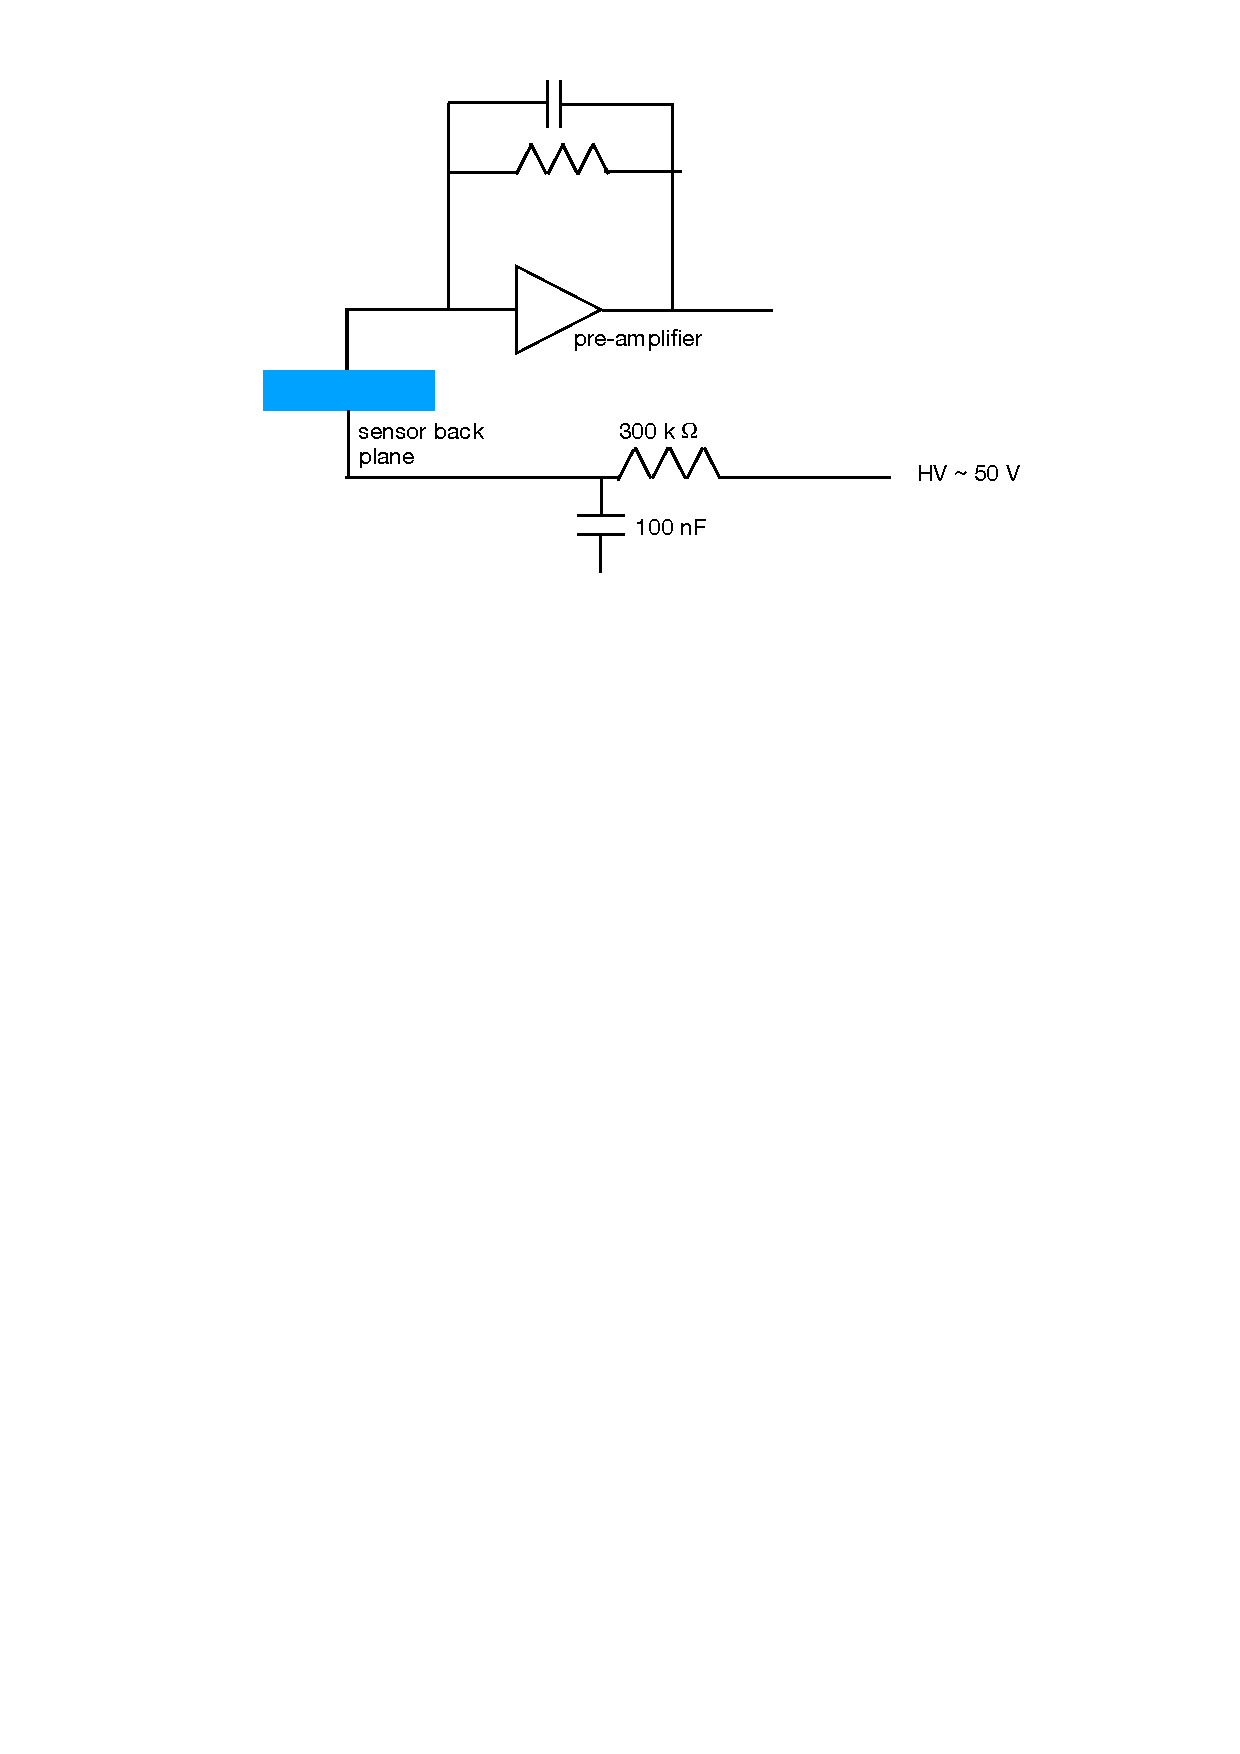
\includegraphics[width=0.6\textwidth]{./graphics/SiliconDiodeCircuit}
  \caption{Silicon detector circuit with low-pass filter, pre-amplifier and silicon diode.}
  \label{fig:SiliconDiodeCircuit}
\end{figure}

%More about the above: The wave supplies a fixed amount of electrons to the pre-amp. That amount can be converted from voltage to charge using the formula:

%\begin{equation}
%  Q = C\cdot V
%\end{equation}

%The capacitance $C$ is going to be the capacitance added to the circuit, in the case of the RMS noise. The charge of the output signal can also be converted into a charge value, but then the capacitance to use must be the sum of the Calib.in capacitance (0.4 pF) and the capacitance that is being added to the circuit.

%Amplitude of the result is 70 percent of the calibration amplitude due to different impedance matching.
%42mv became 32mV after termination (termination = channel at 50 Ohm impedance).

%################################################################################################
%
% Study of the silicon detector
%
%################################################################################################


\section{Study of Silicon detector}

Before integrating the silicon detector inside the rest of the circuit, a few measurements were undertaken to understand its properties: the depletion voltage and the capacitance at depletion. All curves were measured $4$ times, in order to have an estimate of the uncertainty of each measurement.

The IV curve measures the leakage current as a function of voltage and it is useful for measuring the deplation voltage. As it is visible from Figure \ref{fig:IVcurve}, the depletion voltage for this particular silicon diode is of $\approx 50$ V. The current going through the diode at full depletion is of around $-15$ nA. The errorbars are found by taking the standard deviarion between the four measurements performed for each point.

\begin{figure}[h!]
  \centering
  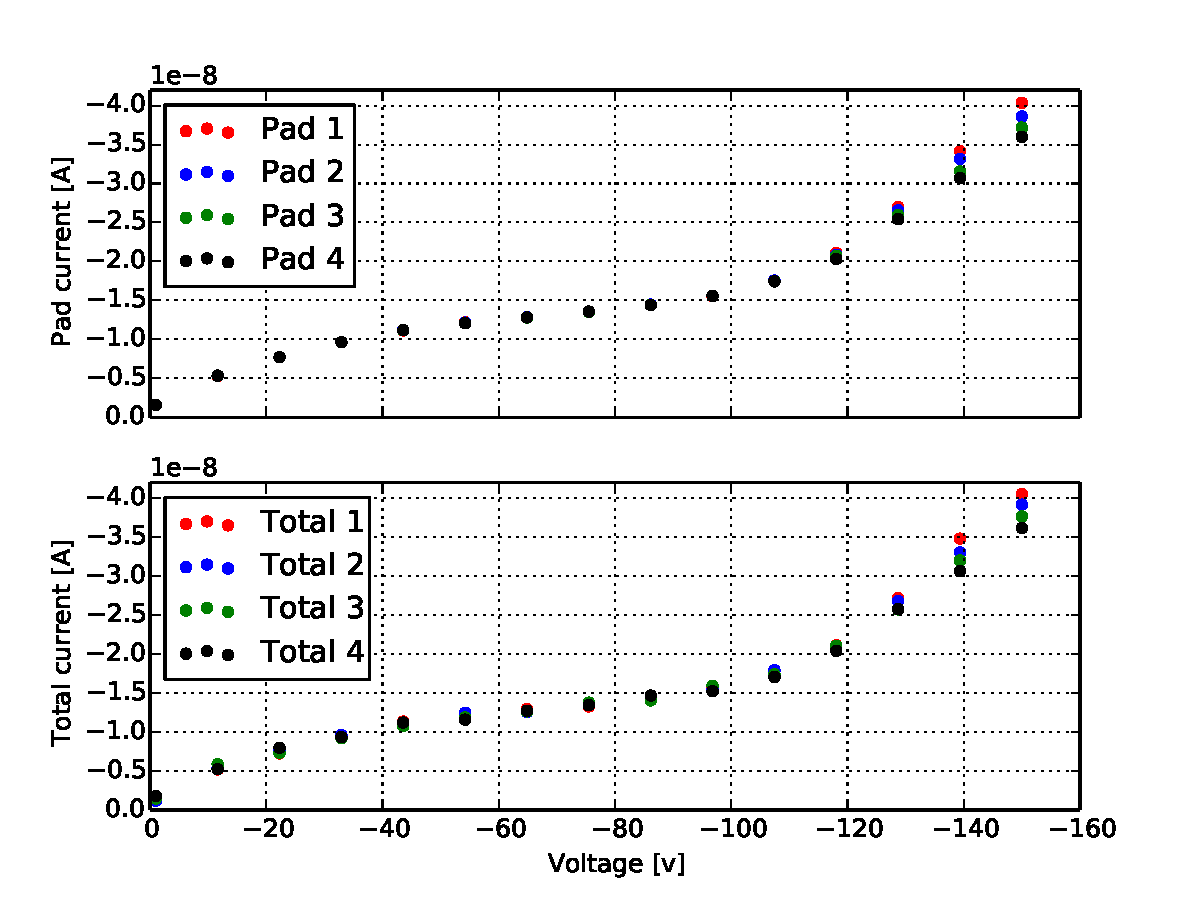
\includegraphics[width=0.8\textwidth]{./graphics/IV_V_vs_A.pdf}
  \caption{IV curve for the silicon detector of p-type. The upper plot shows the current per pad for the $4$ different pads, while the lower plot shows the total current }
  \label{fig:IVcurve}
\end{figure}

The CV curve measures the capacitance of the diode as a function of the voltage and can be seen in Figure \ref{fig:VC_curve_single} for the diode used in this experiment. Before measuring the capacitance of the silicon diode though, we measured the capacitance of the measuring instrument, called "Open needle" in Figure \ref{fig:VC_curve_single}. We then measured the diode capacitance and finally we subtracted the instrument capacitance, to have the actual measurement in red in Figure \ref{fig:VC_curve_single}. Again each measurement was performed $4$ times and the plotted results are the mean of the experiments, while the errorbars are found by calculating the standard derivation of the measurements. In this case, the standard deviation is very small and the errorbars are hence smaller than the data points. The capacitance of the diode at full depletion voltage (above $50$ V) is measured to $11.20 \pm 0.02$ pF, see Figure \ref{fig:VC_curve_single}.

\begin{figure}[t!]
  \centering
  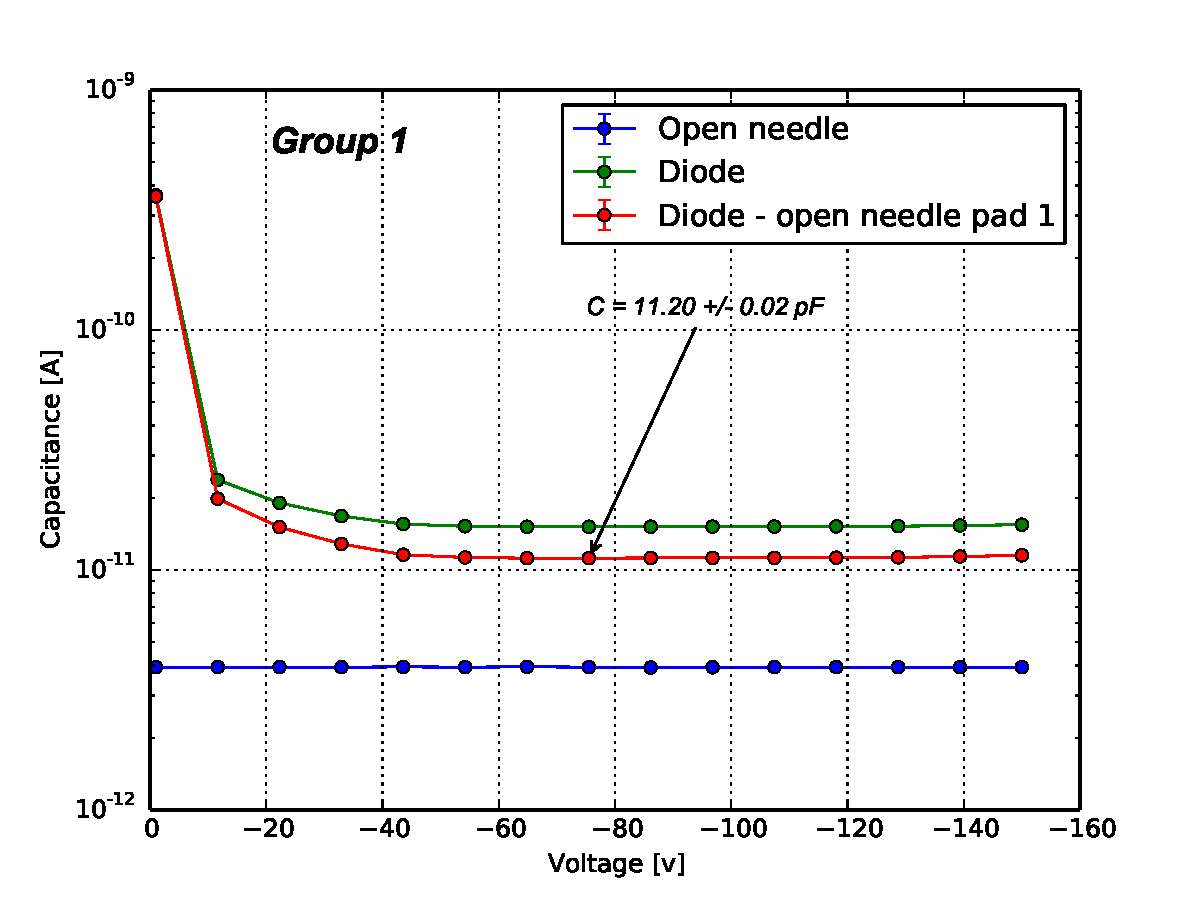
\includegraphics[width=0.8\textwidth]{./graphics/V_vs_C}
  \caption{Parasitic capacitance of the instrument (blue), capacitance of the system plus the silicon diode and capacitance of the diode as a function of voltage.}
  \label{fig:VC_curve_single}
\end{figure}

%################################################################################################
%
% Pre-amplifier calibration curves
%
%################################################################################################

\section{Pre-amplifier calibration}

The response of the pre-amplifier was studied with a calibration signal consisting of a square pulse over the calibration load capacitance, which was between $1$ and $100$ pF. 
Before injecting the square pulse, the noise of the circuit with the different capacitors was measured as the RMS of the noise oscillations. The measurements were recorded and plotted on Figure \ref{fig:Noise_vs_Capacitance}. As it is clearly visible, the noise RMS increases as a function of the input load capacitance.


After feeding the square pulse through the preamplifier, the amplitude and the rise time of the pulse were noted and plotted in Figure \ref{fig:Amplitude_vs_Capacitance} and Figure \ref{fig:RiseTime_vs_Capacitance} respectively. The amplitude decreases as a function of load capacitance, while the rise time increasese, which means that the pulse reacts slowlier and looses some of its power as a functio of capacitance. The rise time was measured by finding the time interval between the $10\%$ and $90\%$ of the rising pulse. 
Additionaly, the measurements with higher capacitances are affected more by the noise, as it is visible by the errorbar size for C = $100$ pF for example. The rise time measurement was fitted to a $2$nd degree polynomial and the resulting paramters are shown in Figure \ref{fig:RiseTime_vs_Capacitance} 

\begin{figure}[htb]
 \centering
  \begin{subfigure}[t]{0.45\textwidth}
  \centering
  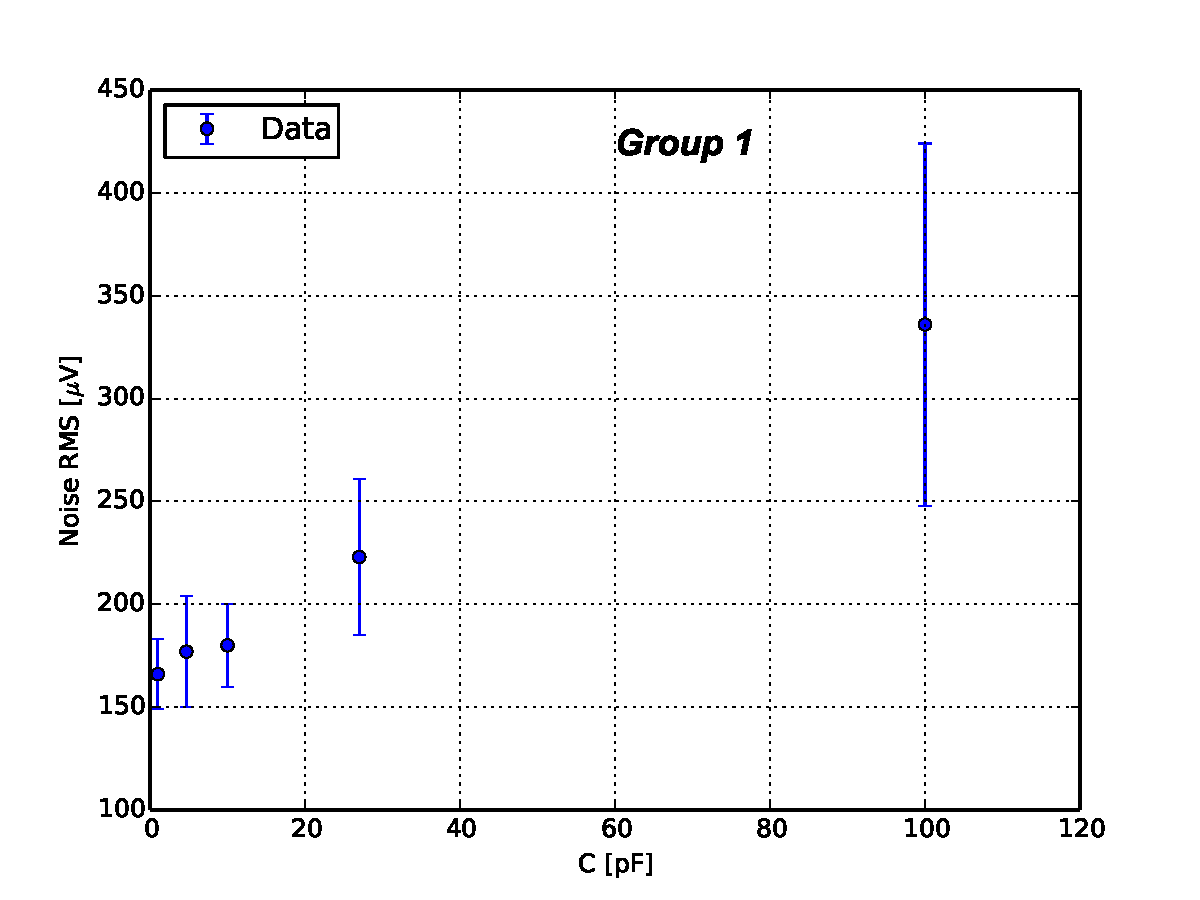
\includegraphics[width=1.2\textwidth]{./graphics/noise_vs_capacitance}
  \caption{Noise RMS vs capacitance measurement}
  \label{fig:Noise_vs_Capacitance}
\end{subfigure}
\hfill
\begin{subfigure}[t]{0.45\textwidth}
  \centering
  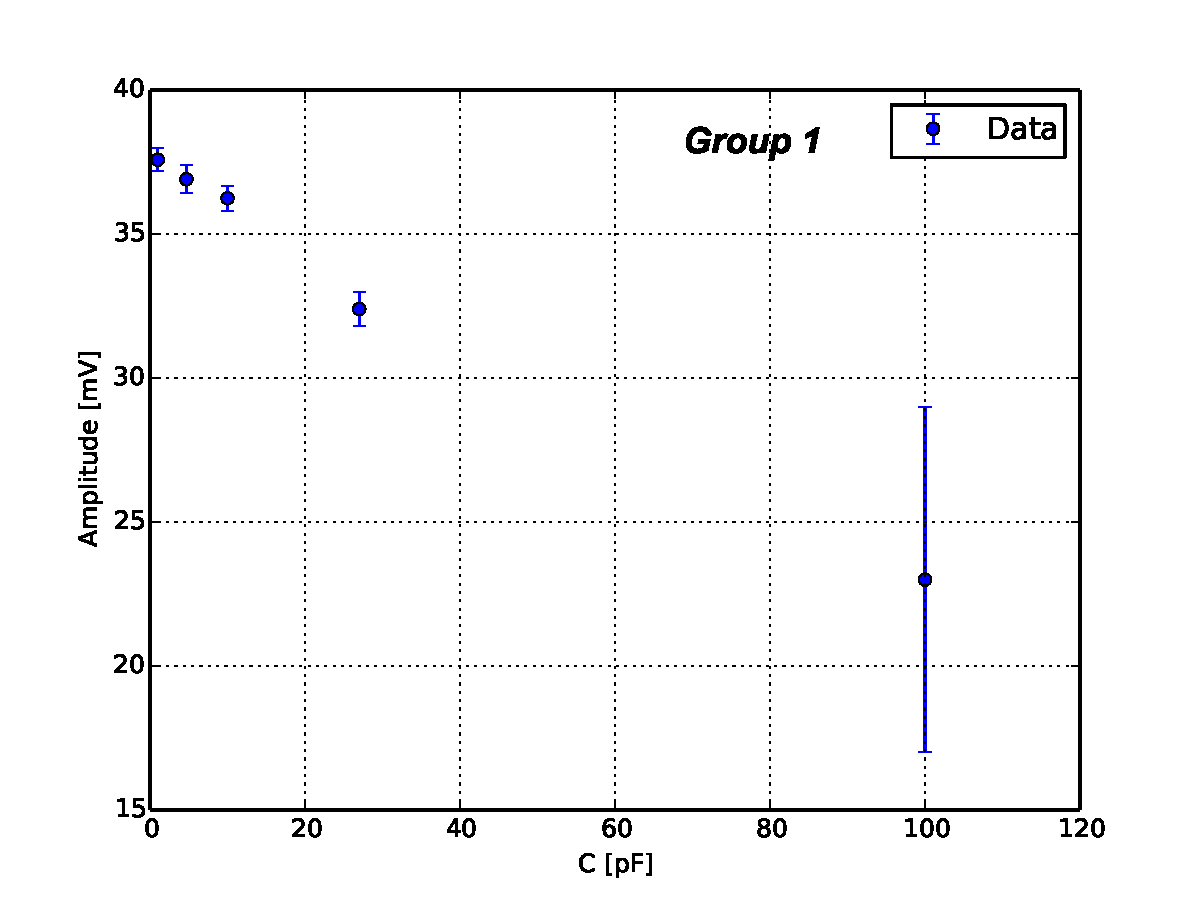
\includegraphics[width=1.2\textwidth]{./graphics/amplitude_vs_capacitance}
  \caption{Amplitude vs capacitance measurement}
  \label{fig:Amplitude_vs_Capacitance}
\end{subfigure}
\caption{Calibration measurements for the pre-amplifier.}
\label{fig:calib_others}
\end{figure}

\begin{figure}[htb]
  \centering
  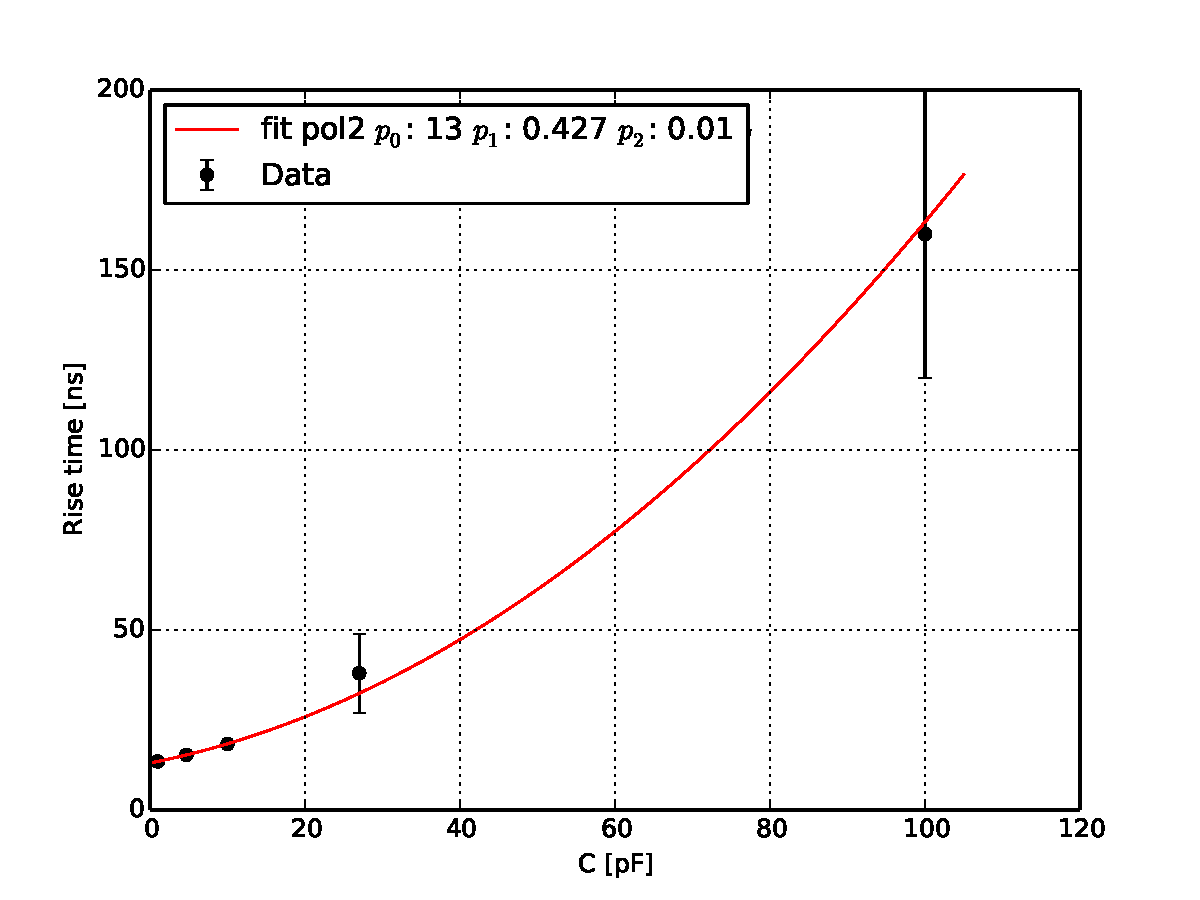
\includegraphics[width=0.8\textwidth]{./graphics/calibration_diode}
  \caption{Calibration of the rise time as a function of capacitance} %%% Add chi2 and errors on the pol2 parameters
  \label{fig:RiseTime_vs_Capacitance}
\end{figure}

%################################################################################################
%
% ENC calibration curve
%
%################################################################################################

\subsection{Equivlent Noise Charge}

The \textit{Equivalent Noise Charge}, or ENC, is the amount of charge one would have to inject into the pre-amplifier in order to match the recorded noise level of the output. In other words, we want to figure out, for a given capacitance, what the RMS noise signal would look like if it were an unamplified input signal. The ENC can be calculated as:
\begin{equation}
ENC = \frac{V_{rms}\cdot C_{calibration}}{G}
\end{equation}
where $V_{rms}$ is the voltage noise RMS, $C_{calibration}$ are the different capacitances used in the calibration procedure and $G$ is the gain.
The gain is given by the ratio of output-to-input voltage:
\begin{equation}
ENC = \frac{V_{in}}{V_{out}}\cdot\left(C_{calibration}\cdot V_{rms}\right)
\end{equation}
where $V_{in}$ is the input voltage of the calibration pulse and $V_{out}$ is the registered output voltage.
During the calibration test, the input voltage is fixed to $20$ mV, so the only thing that varies in this expression should be the capacitance. In practice though, the noise level and the output amplitude depend on the capacitance as well, as shown in Figure \ref{fig:Noise_vs_Capacitance} and \ref{fig:Amplitude_vs_Capacitance}.

\begin{figure}[htb]
  \centering
  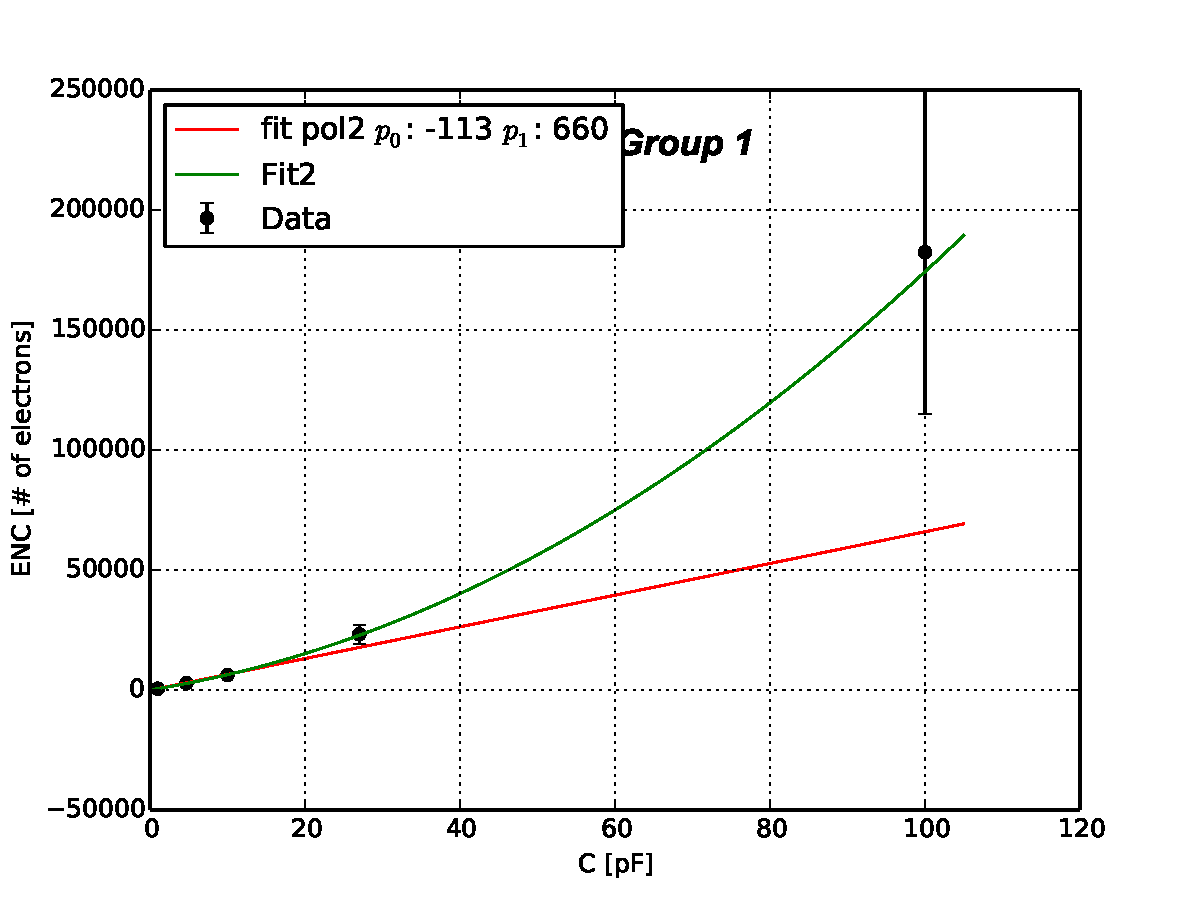
\includegraphics[width=0.8\textwidth]{./graphics/calibrationENC_diode}
  \caption{Calibration of the ENC as a function of capacitance} %%% Add chi2 and errors on the pol2 parameters
  \label{fig:ENC_vs_Capacitance}
\end{figure}

The ENC for the setup with the different capacitors was evaluated and the results can be seen in Figure \ref{fig:ENC_vs_Capacitance}. It is clear that the ENC increases as a function of capacitance and this increase seems linear in the first points, while the last data point, due to the relatively high uncertainty, makes the linear fit less appropriate. The ENC at $0$ pF, given by the intercept in the linear fit, is $-113$ electrons.


%################################################################################################
%
% Results and discussions 
%
%################################################################################################

\section{Results and Discussion}

\begin{figure}[h!]
  \centering
  \begin{subfigure}[t]{0.45\textwidth}
    \centering
    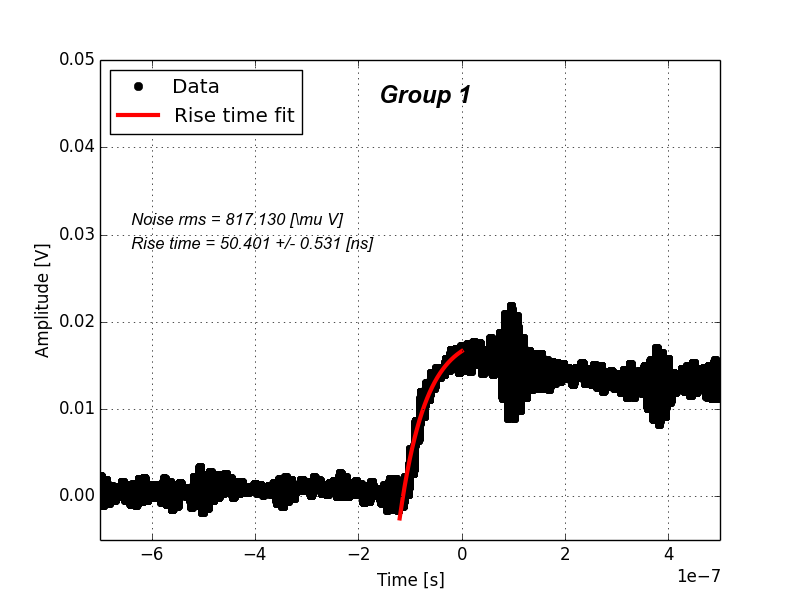
\includegraphics[width=1.1\textwidth]{./graphics/data_0.png}
  \end{subfigure}
  \hfill
  \begin{subfigure}[t]{0.45\textwidth}
    \centering
    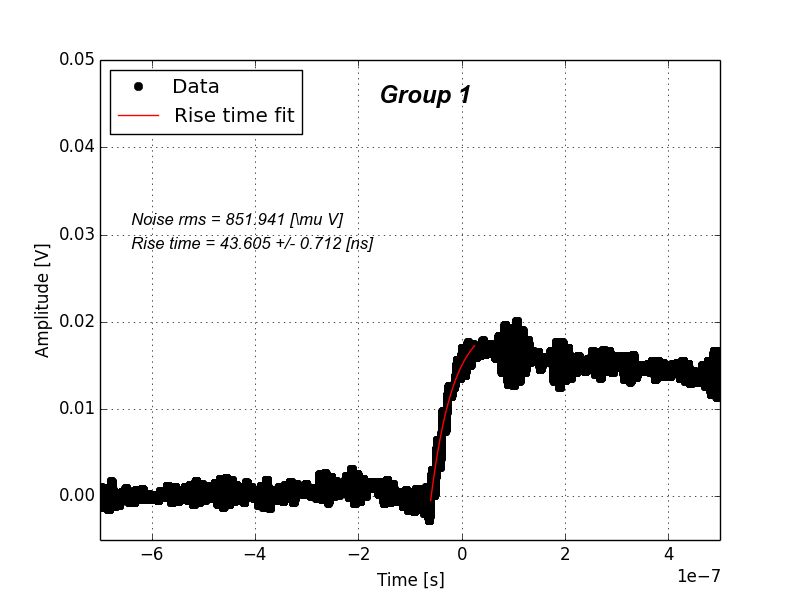
\includegraphics[width=1.1\textwidth]{./graphics/data_1.png}
  \end{subfigure}
  \hfill
  \begin{subfigure}[t]{0.45\textwidth}
    \centering
    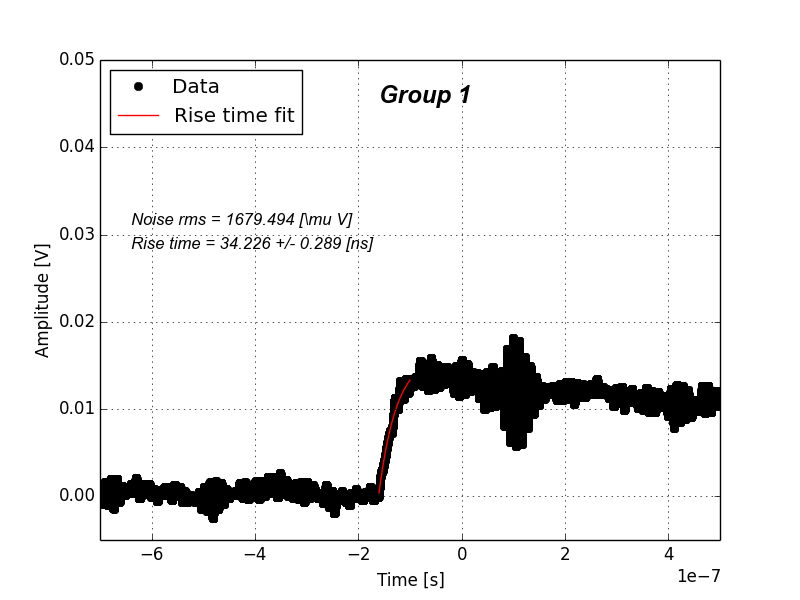
\includegraphics[width=1.1\textwidth]{./graphics/data_2.png}
  \end{subfigure}
  \hfill
  \begin{subfigure}[t]{0.45\textwidth}
    \centering
    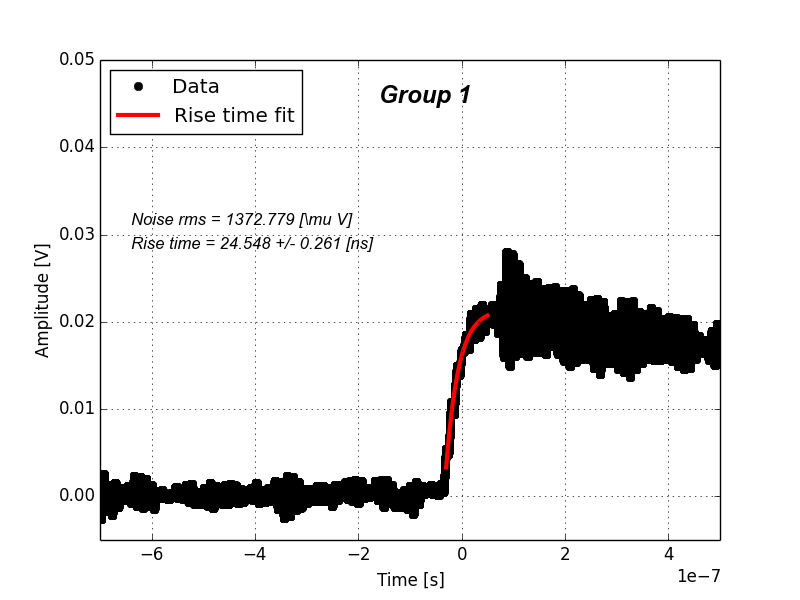
\includegraphics[width=1.1\textwidth]{./graphics/data_3.png}
  \end{subfigure}
  \hfill
  \begin{subfigure}[t]{0.45\textwidth}
    \centering
    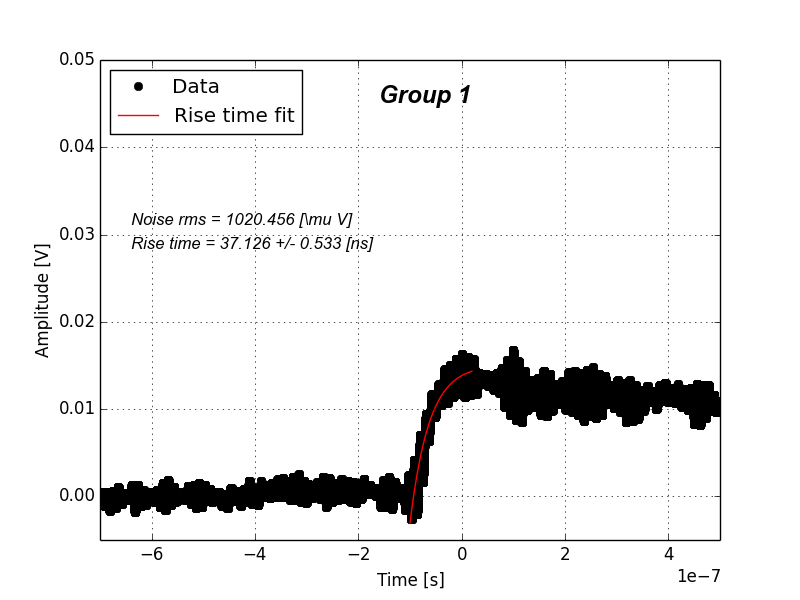
\includegraphics[width=1.1\textwidth]{./graphics/data_4.png}
  \end{subfigure}
  \hfill
  \begin{subfigure}[t]{0.45\textwidth}
    \centering
    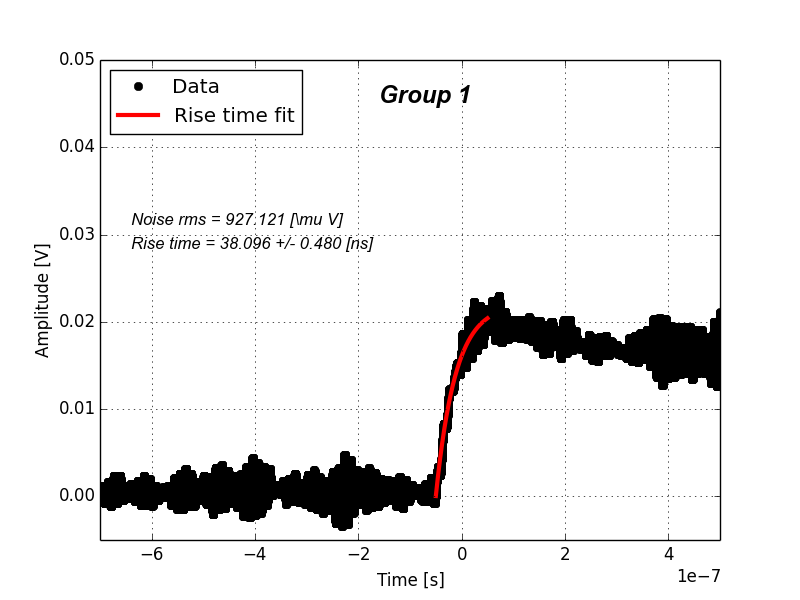
\includegraphics[width=1.1\textwidth]{./graphics/data_5.png}
  \end{subfigure}
\caption{Measurement of the rise time from the Strontium-90 decay. The red line is the fit (see Equation \ref{eq:rise_time}) to the data, while the highlighted green points are the data points used to measure the amplitude and its standard deviation and the blue points are the data used to evaluate the noise RMS}
\label{fig:rise_time_measurement}
\end{figure}
\begin{figure}[h!!]
  \centering
  \begin{subfigure}[t]{0.45\textwidth}
    \centering
    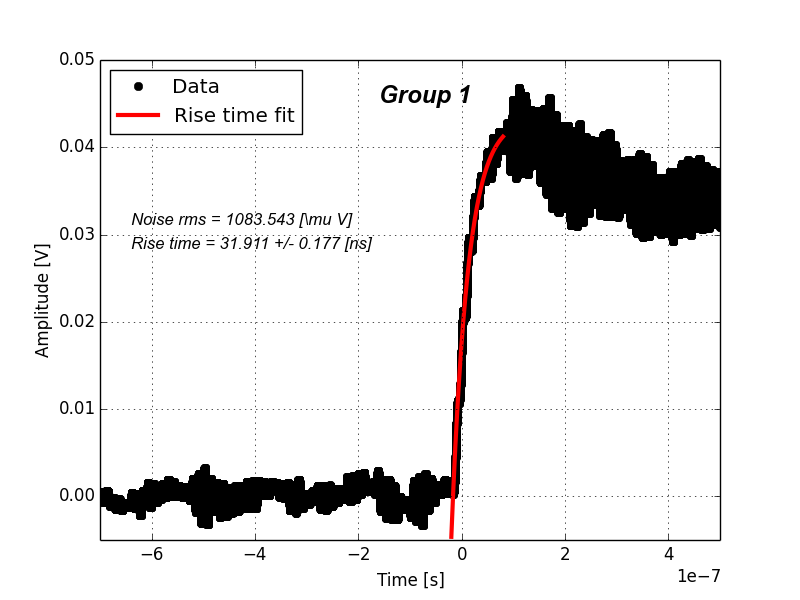
\includegraphics[width=1.1\textwidth]{./graphics/data_6.png}
  \end{subfigure}
  \hfill
  \begin{subfigure}[t]{0.45\textwidth}
    \centering
    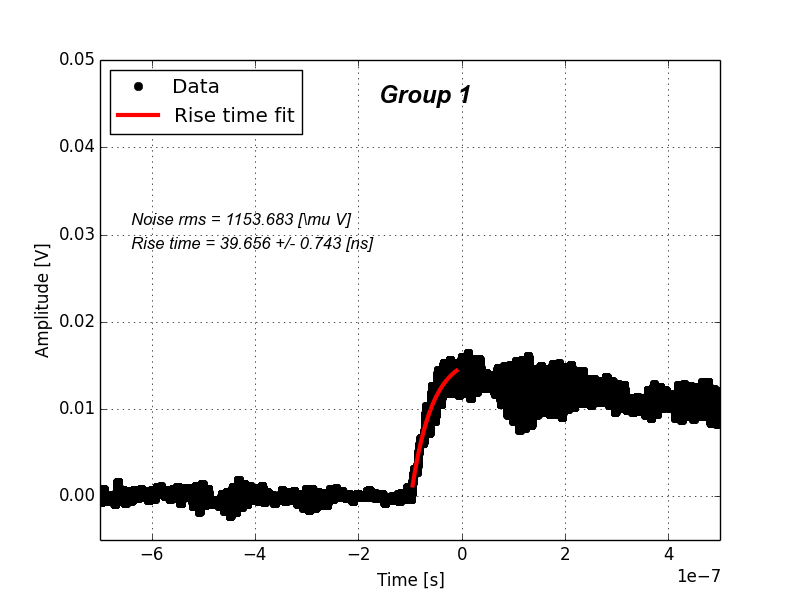
\includegraphics[width=1.1\textwidth]{./graphics/data_7.png}
  \end{subfigure}
  \hfill
  \begin{subfigure}[t]{0.45\textwidth}
    \centering
    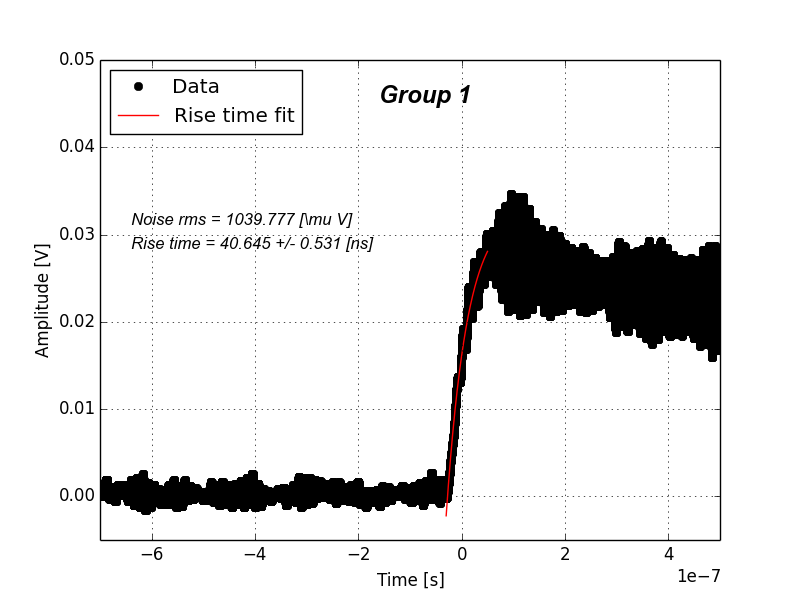
\includegraphics[width=1.1\textwidth]{./graphics/data_8.png}
  \end{subfigure}
  \hfill
  \begin{subfigure}[t]{0.45\textwidth}
    \centering
    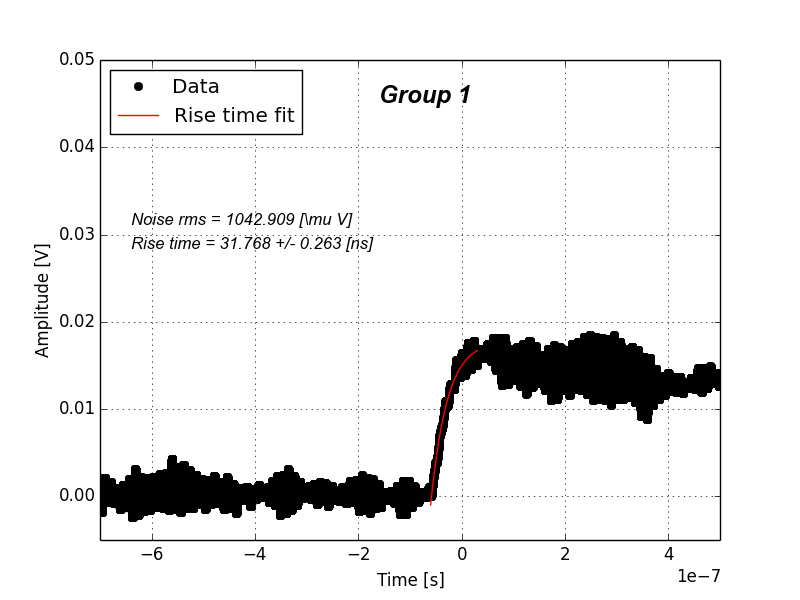
\includegraphics[width=1.1\textwidth]{./graphics/data_9.png}
  \end{subfigure}
  \hfill
  \begin{subfigure}[t]{0.45\textwidth}
    \centering
    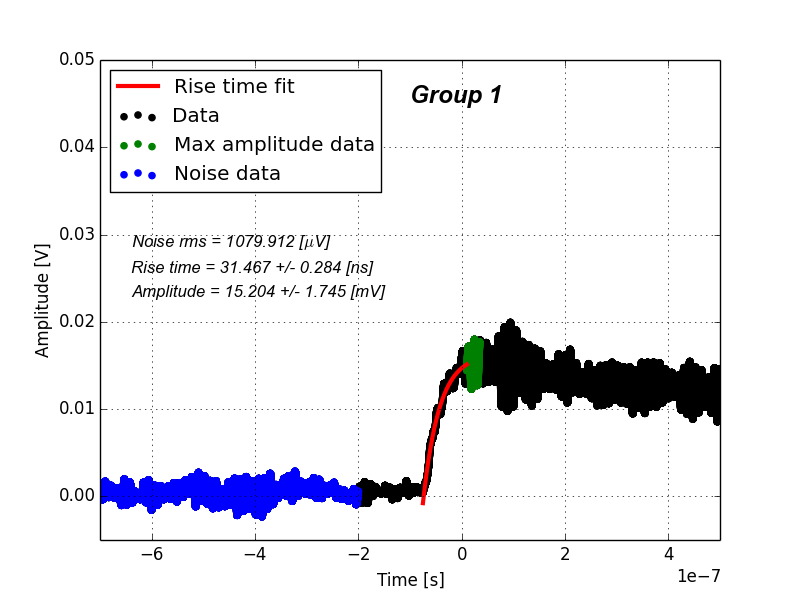
\includegraphics[width=1.1\textwidth]{./graphics/data_10.png}
  \end{subfigure}
  \hfill
  \begin{subfigure}[t]{0.45\textwidth}
    \centering
    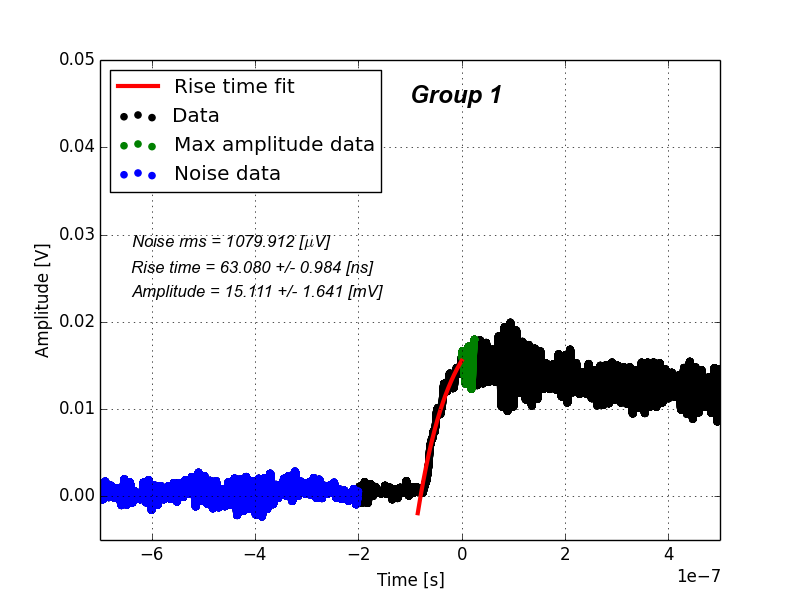
\includegraphics[width=1.1\textwidth]{./graphics/data_11.png}
  \end{subfigure}
\caption{Measurement of the rise time from the Strontium-90 decay. The red line is the fit (see Equation \ref{eq:rise_time}) to the data, while the highlighted green points are the data points used to measure the amplitude and its standard deviation and the blue points are the data used to evaluate the noise RMS}
\label{fig:rise_time_measurement_2}
\end{figure}

After soldering the silicon diode to the rest of the circuit with the pre-amplifier (see Figure \ref{fig:SiliconDiodeCircuit}), we closed the Strontium-90 source and the diode in a box, shielded it with aluminium foil and we connected the pre-amplifier to the $\pm 12$ V source and we applied $\approx 50$ V to diode to fully deplete it. When one of the product decays of the radioactive source hit the diode, it induced a signal, which was observed on the oscilloscope. A few of these signals were saved and are visible in Figure \ref{fig:rise_time_measurement} and \ref{fig:rise_time_measurement_2}. Several measurements were extracted from these data. First of all the noise RMS was measured by taking the standard deviation of all the measured points before the pulse (until Time = $-0.5\mu$ s, which is a cut-off that is valid for all the datasets). The mean noise RMS for all the registered pulses and its uncertainty are $1.0 \pm 0.1$ mV.
The rising pulse is fitted to find the rise time using the equation:
\begin{equation}
  V = V_{0} (1 - \exp^{-t/\tau}) + V_{noise}
  \label{eq:rise_time}
\end{equation}
where $V_{0}$ is the starting amplitude, $V_{noise}$ is the background amplitude and $\tau$ is the rising time. The rising time from the fit and the rising time from the calibration of the pre-amplifier are though not exactly the same rising time, as the first one is measured for the entire rising slope and the second one is measured only between $10\%$ and $90\%$ of the slope. In order to relate the two to each other, this relation exists:
\begin{equation}
t_{r} = \ln(9) \cdot \tau = 2.197 \cdot \tau
\end{equation}
where $t_{r}$ is the time interval between $10\%$ and $90\%$, while $\tau = RC$. 
The mean rise time found with the fits is of $/tau = 38.9 \pm 9.7$ ns and if we multiply this by $2.197$ to get the time interval we get $t_{r} = 85.5 \pm 21.3$ ns. Using the mean rise time, we can extract the capacitance of the silicon detector system by extracting it from the parameters of the calibration curve on Figure \ref{fig:RiseTime_vs_Capacitance}. Given that the rise time calibration curve was fitted with a secon degree polynomial, we use the parameters there to isolate the capacitance term. The statistical uncertainty on the capacitance of the diode system is though evaluated using a Monte Carlo technique with $100.000$ pseudoexperiments. Shortly, we draw $100.000$ different values for each parameter each from a Gaussian distribution, where the mean of the distribution is the value of the parameter and the standard deviation is the uncertainty of the parameter determined by the calibration fits. We solve the equation and find $100.000$ values of the capacitance. The statistical uncertainty is then estimated by taking the standard deviation of the gaussian fitted to the capacitance distribution, see Figure \ref{fig:stat_error_on_C}. The value of the diode system's capacitance is then C = $65 \pm 10$ pF.

\begin{figure}[h!]
  \centering
  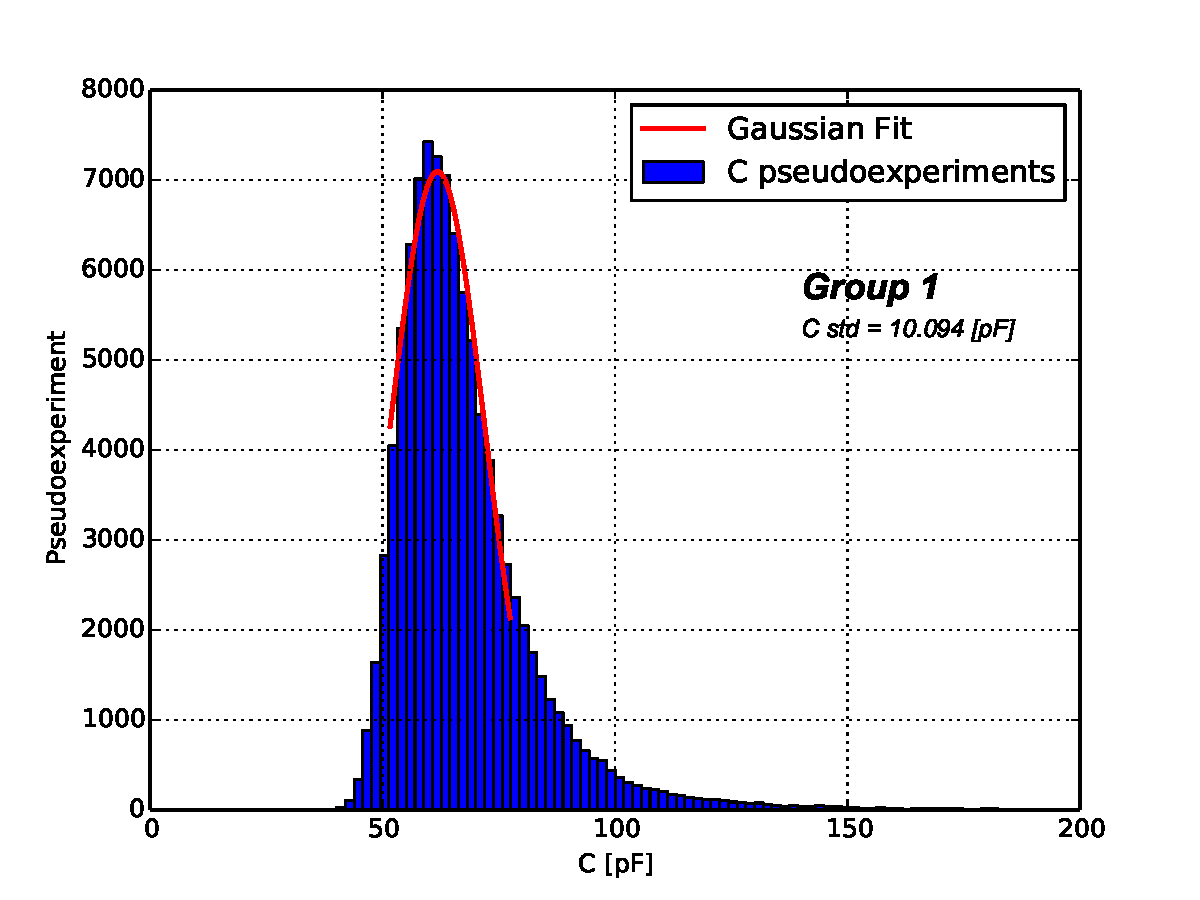
\includegraphics[width=0.8\textwidth]{./graphics/stat_error_on_C_pseudoexperiments}
  \caption{Statistical error on C from Monte Carlo pseudoexperiments}
  \label{fig:stat_error_on_C}
\end{figure}
%Given that the capacitance is found using a second degree coming from the calibration curve, the distribution of the value of the capacitance has a tail in one end. 

Using this extracted value of the capacitance, we can find the ENC of the silicon diode system by again using the parameters in from the ENC calibration curve fit. The uncertainty is calculated using a simple error propagation, as we no longer have to solve a second order degree polynomial. The estimated value of the ENC is $42500 \pm 7700$ electrons.

Finally we extracted the pulse height from the measured Strontium-90 pulses and the values can be found in Figure \ref{fig:rise_time_measurement} and \ref{fig:rise_time_measurement_2}. The calibration pulses and the Strontium-90 pulses were measured with different oscilloscopes, which have different impedances. This results in a $40\%$ difference between the two pulses (with the calibration pulse being the highest). The amplitudes of the recorded Strontium-90 pulses are between $13$ mV and $41$ mV, which multiplied to $1.4$ gives an amplitude range between $18.2$ mV and $57.4$. Given the capacitance of the silicon diode system of $65$ pF, we can extrapolate from the amplitude vs capacitance dataset in Figure \ref{fig:Amplitude_vs_Capacitance} that we would expect an amplitude of between $30$ meV and $20$ meV, which fits the results observed in our experiment.


%################################################################################################
%
% Conclusion
%
%################################################################################################


\section{Conclusion}

In this experiment the preparation and characterisation of a silicon diode detector was observed, its deplation voltage and its capacitance have been measured. The pre-amplifier response was characterized and calibration curves were constructed by analysing the response of the pre-amplifier to a defined input pulse going through a set of dfferent capacitances. After connecting the diode to the pre-amplifier and radiating it with a radioactive source, we coule measure, through the generated pulses by the detected charge, the diode system capacitance and ENC.

















\end{document}
